




\newpage

%----------------------------------------------------------------------------------------

\section{An interdisciplinary approach to morphogenesis}{Une approche interdisciplinaire de la morphogenèse}

\label{sec:interdiscmorphogenesis}


%----------------------------------------------------------------------------------------




\bpar{
A first crucial step is a clarification of what is meant by the term of morphogenesis. Central brick in our constructions, it is indeed crucial to give it a rigorous and clear structure. The approach taken here is aimed at being \emph{interdisciplinary}, in the sense that it takes as an objective to construct a synthetic knowledge implying the different disciplines included\footnote{The approach is slightly different from the effort regarding co-evolution done in~\ref{sec:epistemology}, which proposed a multidisciplinary review but constructed a definition tailored for territorial systems. The work here is the consequence of an interdisciplinary collaboration and is aimed at being more integrative.}, and is therefore aimed as being broad (covered disciplines), deep (depth in each discipline\footnote{Naturally not in the sense of the current knowledge fronts, but in the sense of a non-vulgarized description. The issue is to capture the depth of the discipline while remaining accessible to an interdisciplinary audience.}) and synthetic (integration resulting from it). 
}{
Une première étape essentielle est la clarification de ce qui est entendu par le terme de morphogenèse. Brique essentielle de nos constructions, il est en effet crucial de lui donner une armature rigoureuse et claire. La démarche prise ici est voulue \emph{interdisciplinaire}, au sens où elle se pose comme objectif de construire une connaissance synthétique à partir des disciplines abordées\footnote{Nous nous différentions ici de l'effort concernant la co-évolution mené en~\ref{sec:epistemology}, qui proposait une revue multidisciplinaire mais construisait une définition propre aux systèmes territoriaux. Le travail ici est issu d'une collaboration interdisciplinaire et s'inscrit dans une logique plus intégrative.}, et se veut donc à la fois large (disciplines couvertes), profonde (profondeur dans chaque discipline\footnote{Bien sûr pas au sens d'un compte rendu des fronts de connaissance actuels, mais d'une présentation non vulgarisée. Il s'agit de capter la profondeur de la discipline tout en restant accessible à une audience interdisciplinaire.}) et synthétique (intégration en résultant).
}


\bpar{
The notion of morphogenesis seems to play an important role in the study of a broad range of complex systems. If the concept was introduced in embryology to design growth of organisms, it was rapidly used in various fields, e.g. urbanism, geomorphology and even psychology. However, the use of the concept seems generally fuzzy and to have a field-specific definition for each use. We propose in this section an epistemological study, starting with a broad interdisciplinary review and extracting essential notions linked to morphogenesis across fields. We propose a broad overview, within the spirit of an applied perspectivism such as described in section~\ref{sec:epistemology}, to produce concepts as much generic and broad as possible. This allows to build a consistent general meta-framework for morphogenesis. Further work may include concrete application of the framework on particular cases to operate interdisciplinary transfers of concepts, and quantitative text analysis to strengthen qualitative results.
}{
Le concept de morphogenèse semble jouer un rôle important dans l'étude d'une large gamme de systèmes complexes. S'il a été introduit initialement en embryologie pour désigner la croissance des organismes, il a été rapidement utilisé dans différentes disciplines, e.g. l'urbanisme, la géomorphologie, et même la psychologie. Toutefois, l'utilisation du concept semble généralement floue et avoir une définition spécifique à chaque champ pour chacune de ses utilisations. Nous menons dans cette section une étude épistémologique, commençant par une revue interdisciplinaire large puis en extrayant les notions essentielles liées à la morphogenèse dans chaque champ. Nous prenons le parti d'une vision croisée, dans l'idée d'un perspectivisme appliqué comme introduit en section~\ref{sec:epistemology}, pour obtenir des concepts aussi génériques et larges que possible. Cela permet de construire un méta-cadre général consistent pour la morphogenèse. Des applications peuvent inclure une application concrète du cadre sur des cas particuliers pour opérer un transfert interdisciplinaire de concepts entre disciplines.
}



\paragraph{Context}{Contexte}



\bpar{
During every historical period, people use the main technological advance as a metaphor to explain other phenomena in nature. First, nature was mechanical, then electrical, and now computational. Here, we suggest that taking an alternative metaphor might allow us to better study some properties of a system, and study how the concept of morphogenesis that originated in the study of developmental biology, can be used across systems. Morphogenesis is a very powerful metaphor that is distinct from the previous three that have been very popular in history. Unlike the mechanical, electrical or computational explanations of nature, morphogenesis is not a human designed process. Morphogenesis emphasizes the role of change and growth, rather than a static state. As \cite{thompson1942growth} already pointed out, ``\textit{natural history deals with ephemeral and accidental, not eternal nor universal things}''. The goal of our exercixse is to study three questions: (i) how is morphogenesis defined in different fields?; (ii) are there fields that use approaches and concepts that embody the notion of morphogenesis but do not use the word ?; (iii) to what extent an approache studying morphogenesis can be applied across different fields? A similar effort is described in~\cite{bourgine2010morphogenesis}, but it consists more of a collection of viewpoints from subjects that can be related to morphogenesis rather than an epistemological reconstruction of the notion as we propose to do. Furthermore, examples are far from exhausted and our review is thus complementary.
}{
Durant chaque période historique, l'avancée technologique principale a été utilisée comme une métaphore pour expliquer d'autres phénomènes de la nature. D'abord, la nature a été mécanique, puis électrique, et à présent computationnelle. Ici, nous suggérons qu'une métaphore alternative peut permettre de mieux étudier les propriétés d'un système, et ainsi comprendre comment le concept de morphogenèse qui a trouvé son origine en biologie du développement, peut être utilisé pour d'autres types de systèmes. La morphogenèse est une métaphore très puissante qui est bien distincte des trois précédentes qui ont été très populaires dans l'histoire. Ainsi, contrairement aux explications mécaniques, électriques ou computationnelles de la nature, la morphogenèse n'est pas un processus conçu par l'homme. La morphogenèse met l'accent sur le rôle du changement et de la croissance, plutôt qu'un état statique. Comme \cite{thompson1942growth} mentionnait déjà, ``\textit{l'histoire naturelle traite de l'éphémère et les accidents, pas par des choses éternelles ou universelles}''. Le but de notre exercice est de répondre à trois questions : (i) comment la morphogenèse est définie dans différents champs ; (ii) existe-t-il des champs qui utilisent des approches et concepts incluant la notion de morphogenèse mais sans utiliser le terme ; (iii) dans quelle mesure les approches étudiant la morphogenèse peuvent-elles être transférées entre les champs ? Un effort similaire a été mené par~\cite{bourgine2010morphogenesis} mais consiste plus en une collection de points de vue de sujets liés à la morphogenèse plutôt qu'une reconstruction épistémologique de la notion comme nous proposons de faire. De plus, les exemples sur ce sujet sont loin d'être épuisés et notre revue est pour cela complémentaire.
}



\bpar{
In the context of our global problematic, this work will allow us first to consider consistent territorial systems through the assumption of existing morphogenetic subsystems, and secondly to link territories and networks by the intermediary of the crucial link between form and function that we will develop below.
}{
Dans le cadre de notre problématique globale, cet effort nous permettra d'une part de considérer des systèmes territoriaux cohérents par l'hypothèse de l'existence de sous-système morphogénétiques, et d'autre part de lier territoires et réseaux par l'intermédiaire du lien crucial entre forme et fonction que nous allons développer ci-dessous.
}


\bpar{
The rest of this section is organized as follows: we first provide am autonomous review of the notion of morphogenesis across various fields, ranging from biology to social sciences, psychology and territorial sciences. A synthesis is then made and a framework as general as possible proposed. We finally discuss further developments and potential application of this epistemological analysis.
}{
La suite de cette section est organisée de la façon suivante : nous produisons d'abord une revue autonome de la notion de morphogenèse pour différents champs, s'étendant de la biologie aux sciences sociales, la psychologie et les sciences territoriales. Une synthèse est ensuite faite et un cadre aussi général que possible proposé. Nous discutons finalement des développements futurs et des applications potentielles de cette analyse épistémologique.
}




\subsection{Reviews}{Revues}


\bpar{
We propose a broad overview of the way the notion of morphogenesis if used in field that are a priori rather far from each other. Our review does not pretend to be exhaustive and we do not use any systematic method, the idea being to invoke and cross various relevant conceptions of the notion.
}{
Nous proposons un aperçu large de la manière dont est utilisée la notion de morphogenèse dans des domaines a priori très éloignés. Notre revue ne se prétend pas exhaustive et nous n'utilisons pas de méthode systématique, l'idée étant de mobiliser et de croiser différentes conceptions pertinentes de la notion.
}


\subsubsection{Developmental Biology}{Biologie du développement}


\bpar{
In developmental biology, morphogenesis refers to the mechanisms of how an organism acquires its shape and different functional units, starting from only one cell. Generally, these mechanisms need to work reliably in order to guarantee similar outcomes for every individual. This often requires cells to know their position relative to some reference frame, in order to differentiate, i.e, take a specific function, or to decide whether or not to divide\footnote{The growth of an organism is entirely done through cellular divisions, starting from an initial egg cell. A mature organism is continuously renewed through this uninterrupted division.}, what is a crucial stage in growth. The following part describes models that have been applied in developmental biology.
}{
En biologie du développement, la morphogenèse fait référence aux mécanismes conduisant un organisme à acquérir sa forme et différentes unités fonctionnelles, en partant d'une unique cellule. De manière générale, ces mécanismes doivent être fiables pour garantir une issue similaire pour chaque individu. Cela suppose que les cellules connaissent leur position par rapport à un cadre de référence afin de se différencier, c'est-à-dire prendre une fonction particulière, ou pour décider si elles doivent se diviser\footnote{La croissance d'un organisme a lieu entièrement par division cellulaires, à partir d'une cellule oeuf initiale. Un organisme mature se renouvelle en continu par cette division ininterrompue.} ou non, ce qui est une étape cruciale lors de la croissance. Nous décrivons par la suite les modèles qui ont été appliqués en biologie du développement.
}


\paragraph{Reaction-diffusion mechanisms}{Mécanismes de réaction-diffusion}

\bpar{
Alan Turing used the term reaction-diffusion system in his seminal 1952 paper 'The Chemical Basis of Morphogenesis' to describe simple patterning in a theoretical ring of cells~\cite{turing1952chemical}. Even though this work is now considered one of the most fundamental contributions to the field of pattern formation, it took many years until his work started getting recognition as an actual model for biological systems. \cite{gierer1972theory} has later suggested to use similar models also for intracellular polarity, a ubiquitous phenomenon in biology in which a cell establishes and maintains two different regions within itself. These reaction diffusion networks are one example of the emergence of patterns from a homogeneous state. Using this framework we can recapitulate many pattern formation mechanisms in development, such as coloration or segmentation. These larger scale patterns are generated by the interaction of a few species of chemicals, each chemical species also undergoing a diffusion, production and degradation. Thus it is possible to represent this model using a system of partial differential equations, and certain parameters will generate stable patterns from homogeneous initial condition, where random perturbations are amplified by the system. With only a few molecular species, very complex patterns can be formed~\cite{kondo2010reaction}. One of the most studied reaction-diffusion model capable of producing stable patterns comprises of two types of molecules, one activator and one repressor. The difference in diffusion rate between the two molecules is what amplifies random noise in the system~\cite{gierer1972theory}. The system the most studied at the origin of a coloration corresponds to the reactions responsible from the yellow-black stripes in the Zebrafish~\cite{nakamasu2009interactions}. The emergence of cell polarity is explained in some yeasts by a similar mechanism~\cite{goryachev2008dynamics}. Examples implying function such as body segmentation in \textit{Drosophila melanogaster} usually involves a more complex system than the two previously discussed examples to ensure the robustness of the emergence of these functions.
}{
Le terme de réaction-diffusion avait été utilisé par \noun{Alan Turing} dans son article séminal de 1952~\cite{turing1952chemical}, pour décrire l'émergence de motifs dans un anneau théorique de cellules. Bien que ce travail soit aujourd'hui reconnu comme l'une des contributions les plus fondamentales dans le champ de la formation de motifs, il a fallu des années pour qu'il trouve une reconnaissance comme modèle effectif pour les systèmes biologiques. \cite{gierer1972theory} a plus tard suggéré d'utiliser des modèles similaires pour expliquer la polarité intracellulaire, qui correspond à la capacité d'une cellule à différencier des zones dans son intérieur. Ces réseaux de réaction-diffusion sont un exemple de l'émergence de motifs à partir d'un état homogène, parmi d'autres comme la coloration ou la segmentation. Ces motifs à grande échelle sont générés par l'interaction entre un petit nombre d'espèces chimiques, chacune suivant une diffusion, une production et une dégradation. Il est ainsi possible d'utiliser des systèmes d'équations aux dérivées partielles, pour lesquelles certains paramètres généreront des motifs stables à partir de conditions initiales homogènes, où les perturbations aléatoires sont amplifiées par le système. Des motifs complexes peuvent être produits à partir d'un nombre très restreint d'espèces~\cite{kondo2010reaction}. L'une des réactions capables de produire des motifs stables les plus étudiées comporte deux types de molécules, un activateur et un répresseur. La différence dans le taux de diffusion entre les deux molécules est responsable de l'amplification du bruit dans le système~\cite{gierer1972theory}. Le système à l'origine d'une coloration le plus étudié correspond aux réactions responsables des rayures jaunes et noires du poisson zèbre~\cite{nakamasu2009interactions}. L'émergence de la polarité cellulaire est expliquée chez certaines levures par un mécanisme similaire~\cite{goryachev2008dynamics}. Des exemples impliquant des fonctions comme la segmentation du corps de \textit{Drosophila melanogaster} impliquent des réseaux d'espèces chimiques bien plus complexes pour assurer la robustesse de l'émergence de ces fonctions.
}


\paragraph{The French Flag Model}{Le modèle French Flag}

\bpar{
In a similar way, the French Flag model was initially conceived to explain differentiation of cells in a regular fashion~\cite{Wolpert1969}. The model assumes a graded concentration of a protein, generally called the morphogen, to which tissue cells will react differently depending on its level (thus the flag stripes). Such a gradient must be produced through a diffusion, originating from a source, completed by a stabilisation mechanism implying a sink or a local degradation within the tissue (mechanisms reviewed by~\cite{Rogers2011}). The gradient can then be used locally in a linear way (for example by increasing the expression of a gene linearly with morphogen concentration) or switch-like by local feedback mechanisms. According to~\cite{Wolpert2011}, none of these systems is actually well understood, but empirical evidences of their existence are clear at a large enough granularity, since gradients are indeed observed within a certain number of species. The experiments which are necessary for their exact confirmation are indeed very difficult and within the reach of the current state-of-the-art for most (as they require precise \emph{in vivo} measures of the mobility and decline of given molecules).
}{
De façon similaire, le modèle French Flag a été conçu initialement pour expliquer la différentiation des cellules de manière régulière~\cite{Wolpert1969}. Le modèle suppose un gradient de concentration d'une protéine, généralement appelée le morphogen, auquel les cellules d'un tissu réagiront différemment selon leur niveau (d'où les rayures du drapeau). Un tel gradient doit être produit par une diffusion, à partir d'une source, complété par un mécanisme de stabilisation impliquant un puits ou une dégradation locale dans le tissu (mécanismes qui sont passés en revue par \cite{Rogers2011}). Le gradient peut ensuite être utilisé localement de manière linéaire (l'expression d'un gène variant de manière linéaire par exemple) ou par seuils grâce à des boucles de rétroaction locales. D'après \cite{Wolpert2011}, aucun de ces systèmes n'est parfaitement bien compris, mais les preuves empiriques de leur existence sont claires à une granularité assez grande, puisque les gradients sont effectivement observés chez un certain nombre d'espèces. Les expériences nécessaires pour leur vérification exacte sont en effet très difficiles et encore hors de portée pour la plupart (car supposent des mesures précises \emph{in vivo} de la mobilité et du déclin de molécules données).
}

\paragraph{Intra-cellular forces}{Forces inter-cellulaires}


\bpar{
Cellular rearrangements are often driven by intracellular forces~\cite{Heisenberg2013}, which are then mediated between cells via modulable cell-cell junctions. This phenomenon can lead to a seemingly fluid behavior when an external stress is applied for a given period. On shorter timescales, however, cells exhibit an elastic response, assuming their previous shape if an intermittent external force is no longer present. For the tissue to change in form, occur dome divisions, cell deaths, cell extrusion, or intercalations~\cite{Guillot2013}. An example of a well-studied tissue shape change can be also found in \textit{Drosophila melanogaster}. In this case cells that initially form a flat layer become a long furrow by constricting their cell membrane area on one side~\cite{Lecuit2007}.
}{
Les réagencements cellulaires sont souvent conduits par des forces physiques intracellulaires~\cite{Heisenberg2013}, qui sont ensuite transmises entre cellules, par des jonctions intercellulaires modulables. Ce phénomène peut conduire à un comportement quasi-fluidique lorsqu'un stress extérieur est appliqué pour une certaine durée. À de plus petites échelles temporelles, les cellules gardent cependant un comportement élastique et gardent leur forme lorsqu'aucune force extérieure n'est appliquée. Pour que le tissu change de forme, ont lieu des divisions, morts, extrusions ou intercalages de cellules~\cite{Guillot2013}. Un exemple de dynamique de tissu bien étudiée s'observe chez \textit{Drosophila melanogaster} également. Dans ce cas, des cellules formant initialement une couche plate deviennent un long sillon en contractant la membrane cellulaire d'un coté~\cite{Lecuit2007}.
}


\bpar{
These considerations are both far and close to our general problematic: there exists for example bio-mimetic models applied to urban systems, such as for the generation of a transportation network~\cite{tero2010rules}\footnote{See also a recent initiative by biologists constructing an interdisciplinary project aiming at applying the complex principles of the complex spatial organisation of proteins to the urban space, which has been made concrete through the conference ``Optimized management of space: from cities to natural systems'' in December 2017:  : \url{https://gopro2017.sciencesconf.org/}.}.
}{
Ces considérations sont à la fois lointaines et proches de notre problématique générale : il existe par exemple des modèles bio-mimétiques appliqués aux systèmes urbains, comme pour la génération d'un réseau de transport~\cite{tero2010rules}\footnote{Voir aussi une initiative récente par des biologistes montant un projet interdisciplinaire visant à appliquer les principes complexes d'organisation spatiale complexe des protéines à l'espace urbain, qui s'est concrétisée dans la conférence ``Gestion optimisée de l'Espace : des villes aux systèmes naturels'' en décembre 2017 : \url{https://gopro2017.sciencesconf.org/}.}.
}


\subsubsection*{Artificial Life}{Artificial Life}


\bpar{
The notion of \emph{Programmable Self-assembly} seems in \emph{Artificial Life}\footnote{In the sense of the proper scientific field, leaded for example by the \emph{International Society for Artificial Life} (see \url{http://alife.org/}).} to be very close from the biological concept of morphogenesis: \cite{crosato2014self} notices in a broad review that ``\textit{the best example of \emph{Programmable Self-Assembly} in nature is probably the cell organisation in multicellular organisms, which is encoded by the DNA}''. An important approach in this field is the concept of \emph{Morphogenetic Engineering} introduced by \noun{Doursat}, which focuses on designing complex systems from the bottom-up. A review of the field is done in~\cite{doursat2013review}.
}{
La notion de \emph{Programmable Self-Assembly} semble être en \emph{Artificial Life}\footnote{Au sens du domaine scientifique propre, animé par exemple par la \emph{International Society for Artificial Life} (voir \url{http://alife.org/}).} très proche du concept biologique de morphogenèse : \cite{crosato2014self} note dans une large revue que ``\textit{le meilleur exemple de \emph{Programmable Self-Assembly} dans la nature est probablement l'organisation des cellules en organismes multi-cellulaires, qui est encodée par l'ADN}''. Une approche importante dans ce champ est le concept de \emph{Morphogenetic Engineering} introduit par \noun{Doursat}, qui se concentre sur la conception de systèmes complexes par le bas. Une revue du champ est faite dans~\cite{doursat2013review}.
}

\bpar{
An essential distinction between self-organization and morphogenesis which is introduced in that review is the presence of an \emph{architecture}, in the sense of a macroscopic structure that can be easily isolated and with functional properties~\cite{varenne2015programming} (but that we firstly do not consider as teleonomic~\cite{monod1970hasard} to keep a certain level of generality).
}{
Une distinction essentielle entre auto-organisation et morphogenèse qui y est introduite est la présence d'une \emph{architecture}, au sens d'une structure macroscopique bien discernable ayant des propriétés fonctionnelles~\cite{varenne2015programming} (mais que nous ne considérerons dans un premier temps pas nécessairement téléonomiques~\cite{monod1970hasard} pour garder un certain niveau de généralité).
}

\bpar{
An example of a heterogeneous swarm of particles, yielding complex architectures is described in~\cite{doursat2008programmable}. Processes of local interactions (corresponding in biology to local physical forces) and positional information through gradient propagation are both integrated in the swarm model and allow bottom-up assembly of complex patterns. \cite{sayama2009swarm} develops similar models by adding to it the possibility of an evolution of particle species, directed in real time by the modeler, what allows to effectively orientate the emergent architecture. To what extent these artificial systems are actually close to living systems remains an open question: \cite{Schmickl_2016} exhibit similar swarming rules which lead to the emergence of structures with reproduction properties, and with different functions within a proper ecosystem, which they qualify as ``imitating life''\footnote{We will develop further with more details the necessary concepts to dig further into that affirmation.}. The addition of an environment with its proper properties strongly influences the morphogenetic dynamics, as shown by~\cite{cussat2012synthesis} which combines a chemical reaction layer with an hydrodynamic layer in which the former takes place.
}{
Un exemple d'une nuée hétérogène de particules, produisant des architectures complexes, est décrit dans~\cite{doursat2008programmable}. Les processus d'interactions locales (correspondant en biologie aux forces physiques locales) et l'information de position par la propagation du gradient sont tous deux intégrés dans le modèle et permettent l'émergence de motifs complexes. \cite{sayama2009swarm} développe des modèles similaires en y ajoutant la possibilité d'évolution des espèces de particules, dirigée en direct par le modélisateur, ce qui permet effectivement d'orienter l'architecture émergente. Dans quelle mesure ces systèmes artificiels sont proches de systèmes vivants est une question ouverte : \cite{Schmickl_2016} exhibent des règles de mouvement similaires qui conduisent à l'émergence de structures aux propriétés de reproduction, avec différentes fonctions dans un écosystème propre, qu'ils qualifient comme ``imitant la vie''\footnote{Nous développerons plus en détails plus loin les concepts nécessaires pour creuser cette affirmation.}. L'ajout d'un environnement avec ses propriétés propres influence fortement les dynamiques morphogénétiques, comme montré par~\cite{cussat2012synthesis} qui combine une couche de réaction chimique avec une couche hydrodynamique dans laquelle cette première prend place.
}

\bpar{
The application of these methods to concrete engineering issue begins to be developed with promising results: \cite{Aage:2017aa} use a morphogenesis model for the design of the internal structure of a plane wing and obtains gains in mass up to 5\%, and a final structure very close to forms with similar functions in nature such as a bird wing. In this latest case, bio-mimetism is emergent since it is not assumed within microscopic morphogenesis processes, but is observed at the scale of the whole system.
}{
L'application de ces méthodes à des questions concrètes d'ingénierie commence à être développée avec des résultats prometteurs : \cite{Aage:2017aa} utilise un modèle de morphogenèse pour la conception de la structure interne d'une aile d'avion et obtient des gains de masse allant jusqu'à 5\%, et une structure finale très proche de formes aux fonctions similaires dans la nature comme une aile d'oiseau. Dans ce dernier cas, le bio-mimétisme est émergent puisqu'il n'est pas supposé dans les processus microscopiques de morphogenèse, mais se constate à l'échelle de l'ensemble du système.
}



\subsubsection*{Territorial sciences}{Sciences territoriales}

\bpar{
The concept is used in various disciplines dealing with territories and the built environment: geography, urban planning and design, urbanism, architecture. There does not seem to be a unified view nor theory within these fields, not even within each field itself.
}{
Le concept de morphogenèse est utilisé dans de nombreuses disciplines s'intéressant aux territoires et à l'environnement bâti: géographie, planification et \emph{urban design}, urbanisme, architecture. Il ne semble pas exister de vue unifiée ni de théorie entre les champs ni dans chaque champ lui-même.
}

%%%%%%%%%%%%%%%%%%%%%%%
\paragraph{Built environment}{Environnement bâti}

\bpar{
Architecture and urbanism are disciplines studying human settlements and the built environment at relatively large scale\footnote{We do not include territorial planning, but indeed consider the context of urban projects not broader than the metropolitan scale.}. The theory of Urban Metabolism by \cite{olsen1982urban} links city morphogenesis with urban metabolism and urban ecology. The city is seen as a living organism with different time scales of evolution (the life cycles). The study of urban morphology~\cite{moudon1997urban}, which focuses on morphogenetic processes, is presented as an emerging field in itself, at the interface of geography, architecture and urban planning: this view emphasizes the crucial role of the form in these kind of processes. \cite{burke1972dublin} studies the growth of a particular city (Dublin) during a given period of time, and attributes the evolution of urban morphology to \emph{morphogenetic agents}, i.e. people and developers.
}{
L'architecture et l'urbanisme sont des disciplines étudiant les établissements humains et l'environnement bâti à des échelles généralement grandes\footnote{Nous n'incluons pas l'aménagement du territoire, mais considérons bien le contexte de projets urbains qui ne dépassent jamais l'échelle métropolitaine.}. La théorie du Métabolisme Urbain de \cite{olsen1982urban} relie la morphogenèse de la ville à son métabolisme et à l'écologie urbaine. La ville est vue comme une organisme vivant avec différentes échelles de temps d'évolution (les cycles de vie). L'étude de la morphologie urbaine~\cite{moudon1997urban}, qui s'intéresse aux processus morphogénétiques, est présenté comme un champ émergent en lui-même, à l'interface de la géographie, l'architecture et la planification urbaine : cette vision appuie sur le rôle crucial de la forme dans ce genre de processus. \cite{burke1972dublin} étudie la croissance d'une ville particulière (Dublin) durant une période temporelle donnée, et attribue l'évolution de la morphologie urbaine aux \emph{agents morphogénétiques}, i.e. les habitants et les promoteurs.
}

\bpar{
At another scale, in architecture, a building can be seen as the results of microscopic processes having their own meaning, and a particular architectural style interpreted through the use of a generative shape grammar~\cite{ceccarini2001essai}. This methodology is not far from the work of \noun{C. Alexander}, an architect who produced a theory of design process \cite{mehaffy2007notes}, inspired from computer science and biology and linked in some aspects to complexity. The notion of morphogenesis is in that case however quite loose, as referring to the process of form generation in general, in the same way as~\cite{whitehand1999urban} which studies concrete changes in house forms as witnesses of urban morphogenesis, showing for example that higher density districts are more subject to contagion by minor adaptations by inhabitants.
}{
À une autre échelle, en architecture, un bâtiment peut être vu comme le résultat de processus microscopiques ayant un sens propre, et un style architectural particulier peut être interprété par l'utilisation d'une grammaire générative de formes~\cite{ceccarini2001essai}. Cette méthodologie se rapproche du travail de \noun{C. Alexander}, un architecte ayant produit une théorie des processus de design~\cite{mehaffy2007notes}, inspirée de l'informatique et de la biologie et liée par certains aspects à la complexité. La notion de morphogenèse est dans ce cas cependant assez floue, puisqu'elle se rapporte au processus de la génération de forme en général, de la même façon que~\cite{whitehand1999urban} étudie les changements concrets dans la forme des maisons comme un témoin de la morphogenèse urbaine, montrant par exemple que les quartiers de plus forte densité étaient plus susceptibles à la contagion des adaptations mineures par les habitants.
}

\bpar{
\noun{Dollens} refers to autopoiesis~\cite{dollens2014alan}\footnote{The concept of \emph{autopoiesis} on which we will come back with more details in the following, mainly consists in the ability of a system to be self-sustained as an autonomous network of processes.}, implying a particular case of morphogenesis, to advocate \noun{Turing}'s influence on contemporary design thinking, and to propose a more organic approach to architecture. \cite{desmarais1992premisses} sustains the thesis that human structures carry an abstract morphology, and that it is generated by processes carrying meaning, rejoining the conception by~\cite{ceccarini2001essai}. This echoes with the use of morphogenesis in psychology as we will see further: the elaboration of the concrete form of the artefact is then converging with the cognitive process of agents generating it, and this cognitive process can in itself be understood as a morphogenesis. \cite{levy2005formes} highlights the difficulty to give a proper definition of the term of urban form, and proposes to revisit it by linking the production of the form to the production of meaning within the full dynamic of the system. This positioning partly rejoins the one we will take later to define morphogenesis.
}{
\noun{Dollens} fait référence à l'autopoièse~\cite{dollens2014alan}\footnote{Le concept d'\emph{autopoièse} sur lequel nous reviendrons plus en détail par la suite, consiste principalement en la capacité d'un système de s'auto-entretenir comme réseau autonome de processus.}, impliquant un cas particulier de morphogenèse, pour défendre l'influence de \noun{Turing} sur la pensée contemporaine en design, et pour proposer une approche plus organique de l'architecture. \cite{desmarais1992premisses} soutient que les structures humaines sont porteuses d'une morphologie abstraite, et que celle-ci est générée par des processus porteurs de sens, rejoignant la conception de~\cite{ceccarini2001essai}. Cela fait écho aux usages de la morphogenèse en psychologie comme nous verrons plus loin : l'élaboration de la forme concrète de l'artefact va alors de pair avec le processus cognitif des agents la générant, et ce processus cognitif peut lui-même être compris comme une morphogenèse. \cite{levy2005formes} soulève la difficulté d'une définition propre du terme de forme urbaine, et propose de le revisiter en liant la production de la forme à celle du sens dans l'ensemble de la dynamique du système. Ce positionnement rejoint partiellement celui que nous prendrons plus loin pour définir la morphogenèse.
}





%%%%%%%%%%%%%%%%%%%%%%%
\paragraph{Urban modeling}{Modélisation urbaine}


\bpar{
The literature in modeling urban growth often refers to the growth process as morphogenesis when the scale implied allows to exhibit shape patterns. An example of the emergence of qualitatively different urban functions, based on the Alonso-Mills-Muth model is proposed in~\cite{bonin2012modele}. \cite{bonin2014modelisation} also extends this standard model of urban economics and directly refers to \emph{morphogens}, the substance which diffuse and react in the initial formulation of morphogenesis by \noun{Turing}. This model takes into account population, real estate prices, housing surfaces, employments and endogenous amenities, and simulates the evolution of their spatial distribution and of the resulting urban form.
}{
La littérature de modélisation de la croissance urbaine se réfère souvent au processus de croissance comme morphogenèse quand l'échelle impliquée permet de révéler des motifs de forme. Un exemple de l'émergence de fonctions urbaines qualitativement différenciées, dans un modèle basé sur le modèle d'Alonso-Mills-Muth, est proposé dans~\cite{bonin2012modele}. \cite{bonin2014modelisation} étend également ce modèle standard d'économie urbaine et fait directement référence aux \emph{morphogens}, substance qui diffusent et réagissent dans la formulation initiale de la morphogenèse par \noun{Turing}. Ce modèle prend en compte la population, les prix immobiliers, les surfaces de logement, les emplois et des aménités endogènes, et simule l'évolution de leur distribution spatiale et de la forme urbaine résultante.
}

\bpar{
\cite{makse1998modeling} studies a model of urban growth involving the local urban form. In this case the local spatial correlations induce urban structure when the cities gain new inhabitants. More heterogeneous models imply a coupling between city components and transportation networks. \cite{achibet2014model} describe a model of co-evolution between road network and urban blocks structure. At a smaller scale and involving more abstract functions, \cite{raimbault2014hybrid} couple city growth with network growth, including a local feedback of the form through a density constraint and a global feedback of position through network centrality and accessibility to amenities. These two mechanisms are analogous to local interactions and the diffusion of a global information flow in biology.
}{
\cite{makse1998modeling} étudie un modèle de croissance urbaine impliquant la forme urbaine locale. Dans ce cas les corrélations spatiales locales induisent la structure urbaine quand les villes gagnent de nouveaux habitants. Des modèles plus hétérogènes impliquent un couplage entre les composantes urbaines et les réseaux de transport. \cite{achibet2014model} décrit un modèle de co-évolution entre réseau de rues et la structure des blocs urbains. À une plus petite échelle et impliquant des fonctions plus abstraites, \cite{raimbault2014hybrid} couplent croissance urbaine et croissance de réseau, incluant une rétroaction locale de la forme par une contrainte de densité et une rétroaction globale de la position par la centralité de réseau et l'accessibilité aux aménités. Ces deux mécanismes sont analogues aux interactions locales et à la diffusion du flux d'information global en biologie. 
}

%\comment{\cite{bonin2014modelisation} precedent modele revisité : parallele precis avec les substances morphogenes : reaction diffusion.}

%\comment{le simpopnano comme un modele de morphogenese \cite{louail2009geometrie}}[bof pas vraiment]



%%%%%%%%%%%%%%%%%%%%%%%
\paragraph{Archeology}{Archéologie}


\bpar{
The morphogenesis of past human settlements viewed from Thom's Catastrophe Theory point of view, is introduced by~\cite{renfrew1978trajectory}. Sudden changes (qualitative changes, or regime shifts) have occurred at any time and can be viewed as bifurcations during the morphogenesis process. Another simplified way to see this is to interpret the transition as a change of meta-parameters of a stationary dynamic.
}{
La morphogenèse des établissements humains du passé, vue du point de vue de la théorie des catastrophes de \noun{Thom}, est introduite dans~\cite{renfrew1978trajectory}. Des changement soudains (changement qualitatifs, ou changements de régime) se sont produits à toute époque et peuvent être vus comme des bifurcations durant le processus de morphogenèse. Une autre manière simplifiée de le comprendre est d'interpréter la transition comme un changement des meta-paramètres d'une dynamique stationnaire.
}





\subsubsection*{Social science and psychology}{Sciences sociales et psychologie}

\bpar{
Morphogenesis has been occasionally used as a suitable metaphor to understand different processes in social science and various psychological fields (we will in the following designate the corresponding systems as psychological systems). In developmental psychology for example, the influence of cultural learning processes on behavior are a suitable example~\cite{hart_held_2013}. Regarding clinical psychology, analogies are used for the self-organization of relations with the Self and the Other, and also for dynamics implying creative emergence, which must be fostered for a ``successful'' psychotherapy~\cite{piers_self-organizing_2007}. Moreover, in the field of neuroscience, the structure of brain in itself and the development of neural networks is typically the product of morphogenetic processes~\cite{_issues_2013}. In social psychology, the co-evolution between the individual and society can also be understood through. that approach~\cite{archer_margaret_1999}. The theory by \noun{René Thom} which we will detail later has certainly played a role in the use of this concept in psychology~\cite{de_luca_picione_processes_2016}. Nonetheless, more than a systematic and widespread unity throughout these different fields, we encounter multiple uses that are sometimes discontinuous, and one could argue that the utility of morphogenesis could be more tangible on an epistemological level. This would consist of a shared perception of morphogenesis’s descriptive power to further understand the emergence and structure of various phenomena.
}{
La morphogenèse a été occasionnellement utilisée comme une métaphore efficace pour comprendre différents processus en sciences sociales et dans divers champs de la psychologie (nous désignerons les systèmes concernés par le terme générique de systèmes psychologiques). En psychologie du développement par exemple, l'influence des processus d'apprentissage culturel sur le comportement sont une bonne illustration~\cite{hart_held_2013}. Pour la psychologie clinique, des analogies sont utilisées pour l'auto-organisation des relations avec le Moi et l'Autre, ainsi que pour les dynamiques impliquant l'émergence créative, qui doit être encouragée pour une psychothérapie ``aboutie''~\cite{piers_self-organizing_2007}. D'autre part, en neurosciences, la structure du cerveau en elle-même et la mise en place des réseaux de neurones est typiquement le produit de processus morphogénétiques~\cite{_issues_2013}. En psychologie sociale, la co-évolution de l'individu et de la société peut également être vu par ce prisme~\cite{archer_margaret_1999}. La théorie de \noun{René Thom} que nous détaillerons plus loin a certainement joué un rôle dans l'utilisation de ce concept en psychologie~\cite{de_luca_picione_processes_2016}. Toutefois, au delà d'une unité systématique au travers de ces différents champs, les usages sont plutôt discontinus, et nous pouvons supposer que l'utilité du concept de morphogenèse réside plutôt dans sa portée épistémologique. Celle-ci consisterait dans une perception partagée du pouvoir descriptif de la morphogenèse pour mieux comprendre l'émergence de la structure des divers phénomènes.
}


\subsubsection{Epistemology}{Epistémologie}

\bpar{
Morphogenesis is also used to study science itself: for example~\cite{gilbert2003morphogenesis} studies the evolution of evolutionary developmental biology through the metaphor of morphogenesis. He sees scientific ideas as interacting agents from which emerge new phenotype through differentiation processes, what is designed as the morphogenesis of the field.
}{
La morphogenèse peut aussi être utilisée pour étudier la science elle-même : par exemple~\cite{gilbert2003morphogenesis} étudie l'évolution de la biologie évolutionnaire du développement par la métaphore de la morphogenèse. Il voit les idées scientifiques comme des agents en interaction, desquels émergent de nouveaux phénotypes par des processus de différentiation, qui sont désignés comme la morphogenèse du champ.
}



\subsubsection{History of the notion}{Histoire de la notion}

\bpar{
The study of morphogenesis started with embryology between just before 1930's. This is about the same period at which cellular moves of bacteria have been discovered~\cite{abercrombie1977concepts}. Statistics obtained from Google Books\footnote{See the \emph{Google Books ngram viewer} which allows to visualize the evolution of terms use in time in the full Google Books corpus, available at \url{https://books.google.com/ngrams/graph?content=morphogenesis}.} give the first use of the word morphogenesis in a book is in 1871. The use then saw a large peak in usage between 1907 and1909, and continued to increase in usage until the 1990's before slowing decreasing in usage.
}{
L'étude de la morphogenèse a démarré avec l'embryologie juste avant les années 30. Il s'agit environ de la même période à laquelle les mouvement cellulaires de bactéries ont été découverts~\cite{abercrombie1977concepts}. Les statistiques issues de Google Books\footnote{Voir le \emph{Google Books ngram viewer} qui permet de visualiser l'évolution de l'usage de termes dans le temps dans l'ensemble du corpus Google Books, disponible à \url{https://books.google.com/ngrams/graph?content=morphogenesis}.} donne le premier usage du mot dans un livre en 1871. L'usage montre ensuite un pic d'utilisation entre 1907 et 1909, pour continuer d'augmenter jusqu'en 1990 avant de décroître progressivement.
}


\subsubsection{Putting into perspective}{Mise en perspective}


\bpar{
These journeys through diverse disciplines have already allowed us to unveil key ideas and concepts similar to morphogenesis. We conclude this review with a broader perspective to be more general.
}{
Ces voyages par diverses disciplines nous ont permis déjà de dégager des idées clés et des concepts voisins à la morphogenèse. Nous concluons cette revue par une mise en perspective pour gagner en généralité.
}



\paragraph{A mathematical approach}{Une approche mathématique}


\bpar{
Ren{\'e} Thom developed in \emph{Structural stability and Morphogenesis}~\cite{thom1974stabilite} a theory of system dynamics, the catastrophe theory, which can be specified as understanding the impact of the topological structure of the phase space on system dynamics. We detail the synthesis done by~\cite{petitot2011morphogenetic}, in particular in the case of the specification for dynamical systems. Let $M$ be a differentiable manifold, in which the system state $(\vec{x},\dot{\vec{x}})_w$ is embedded, parametrized by an external control $w\in W$. There exists than a closed set $K\subset W$ called \emph{catastrophe set}. The topological type of $K$ is indeed endogenously determined by system dynamics (in simple cases, it refers to the ``classical'' type of attractors and fixed points usually known: points and limit cycles). When $w$ encounters $K$, the system undergoes a \emph{qualitative} change in its form, what constitutes the basis of \emph{morphogenesis}.
}{
Ren{\'e} Thom a développé dans \emph{Stabilité Structurelle et Morphogenèse}~\cite{thom1974stabilite} une théorie de la dynamique des systèmes, la théorie des catastrophes, qui peut être spécifiée pour comprendre l'impact de la structure topologique de l'espace des phases sur les dynamiques du système. Nous précisons la synthèse qui en est faite par~\cite{petitot2011morphogenetic}, en particulier dans le cas de la spécification aux systèmes dynamiques. Soit $M$ une variété différentielle, dans laquelle l'état du système $(\vec{x},\dot{\vec{x}})_w$ est embarqué, paramétré par un contrôle extérieur $w\in W$. Il existe alors un ensemble fermé $K\subset W$ appelé \emph{ensemble de catastrophe}. Le type topologique de $K$ est en fait déterminé de manière endogène par la dynamique du système (dans les cas simples, il réfère au types ``classiques'' d'attracteurs et points fixes que l'on connait habituellement : points et cycles limites). Quand $w$ rencontre $K$, le système subit un changement \emph{qualitatif} dans sa forme, ce qui constitue la base de la \emph{morphogenèse}.
}


\bpar{
This abstract theory of morphogenesis is independent of the nature of the system studied, its main contribution being to classify local catastrophes that occur during morphogenesis. Differentiation and richness of patterns have thus a geometrical explanation through the topological types of catastrophes. \noun{Thom} notes that at the time of his writing, the study of form has mainly be the focus of biology, but that many applications could be done in physics and geomorphology for example. He formulates the hypothesis that because this implies discontinuities and self-organisation, to which mathematicians were repulsive, this was not applied easily to various fields. We can link this to the rise of complexity approaches, with complexity paradigms that slowly spread in various disciplines, and which the study of morphogenesis seem to have followed.
}{
Cette théorie abstraite de la morphogenèse est indépendante de la nature du système étudié, sa contribution principale étant de classifier les catastrophes locales qui surviennent lors de la morphogenèse. La différentiation et la richesse des motifs ont ainsi une explication géométrique à travers les types topologiques des catastrophes. \noun{Thom} note qu'à cette époque, l'étude de la forme a majoritairement été ciblée par la biologie, mais que de nombreuses applications pourraient être développées en physique et géomorphologie par exemple. Il formule l'hypothèse que parce que cela implique des discontinuités et de l'auto-organisation, à laquelle les mathématiciens étaient réticents, la théorie n'a pas été appliquée facilement à divers champs. Nous pouvons lier cela à l'émergence des approches complexes, avec des paradigmes de la complexité qui se sont progressivement répandus dans diverses disciplines, et l'étude de la morphogenèse semble avoir suivi. 
}


%%%%%%%%%
% Quote from Villani on Morphogenesis (thanks Mario !)
% Morphogenesis as a discipline that is not yet very clearly identified, having still lots of mystery, it is in the intersection between mathematics, chemistry and biology. Typically it is in chemical reactions produced in the development of living beings, where some mathematical models play a role to make structures emerge, so it really makes these 3 intervene (math, chem, biol). And Turing identified that when we put together and at the same time a diffusion phenomenon -with a substance that spreads in an organism- and a chemical reaction, we can end up with instabilities. And for example, these instabilities make the leopard's skin, where you can see black spots, instead of black being evenly distributed. And this incredible article by Turing was a struck of genius, to think that by putting together two stable phenomena -because this chemical reaction is a stable phenomena, and the diffusion is a stable phenomena- one could have an instability. Completely counter-intuitive, but mathematics is precisely that which can permit us to go beyond intuition.


\bpar{
Mathematics, not mentioned that much in our review, are however concerned both as a tool but also as a discipline in itself, since mathematical constructions obtained from questions linked to morphogenesis are research subjects in themselves. As recently recalled \noun{Cedric Villani} in~\cite{villani2017chauvesouris}, ``\textit{morphogenesis is a discipline which is not yet clearly identified and still with many mysteries, at the intersection of mathematics, chemistry and biology, where mathematical models play a role to make the structures emerge}''.
}{
Les mathématiques, peu mentionnées dans notre revue, sont toutefois concernées à la fois comme outil mais aussi comme discipline à part entière, les constructions mathématiques obtenues à partir des questions liées à la morphogenèse sont des sujets de recherche propres. Comme l'a récemment rappelé \noun{Cedric Villani} dans~\cite{villani2017chauvesouris}, ``\textit{la morphogenèse est une discipline pas très bien identifiée ayant toujours un certain nombre de mystères, à l'intersection entre les mathématiques, la chimie et la biologie, où des modèles mathématiques jouent un rôle pour faire émerger les structures}''.
}




\paragraph{Autopoiesis}{Autopoièse}

\bpar{
The concept of autopoiesis, which initially originates from biology, is intimately linked to morphogenesis. In the case of psychological systems, it provides an interpretation of cognition and conscience which depends on the observer. This had impacts in psychology and sociology, such as some theories of systems~\cite{gershenson2015requisite}. Social and phychological systems are then understood as strongly coupled systems, as witnesses language which is a social phenomenon deeply anchored within cognitive manifestations~\cite{seidl_luhmanns_2004}. These approaches also rejoin the views of the self as dynamical and recursive~\cite{pichon_riviere_processus_2004}. The interpenetration of the social and the psychological have an echo in the psychanalytical anthropology of \noun{Freud} which highlights the relations between nevrotic symptoms and socio-cultural phenomena~\cite{freud_totem_1989}.
}{
Le concept d'autopoièse, qui provient initialement de la biologie, est intimement lié à la morphogenèse. Dans le cas des systèmes psychologiques, il fournit une interprétation dépendante de l'observateur de la cognition et de la conscience. Celle-ci a eu des impacts en psychologie et sociologie, comme certaines théories des systèmes~\cite{gershenson2015requisite}. Les systèmes sociaux et psychiques sont alors compris comme des systèmes fortement couplés, comme le témoigne le language qui est un phénomène social profondément ancré dans les manifestations cognitives~\cite{seidl_luhmanns_2004}. Ces approches rejoignent également les visions du sujet comme dynamique et récursif~\cite{pichon_riviere_processus_2004}. L'interpénétration du social et du psychologique trouvent écho chez l'anthropologie psychanalytique de \noun{Freud} qui appuie les relations entre les symptômes de névrose et les phénomènes socio-culturels~\cite{freud_totem_1989}.
}




\bpar{
In its biological sense, it expresses the ability for a system to reproduce itself. A basic characterization is the existence of a semi-permeable boundary produced within the system and the ability to reproduce its components. A more general definition is proposed by~\cite{bourgine2004autopoiesis}\footnote{\textit{``An autopoietic system is a network of processes that produces the components that reproduce the network, and that also regulates the boundary conditions necessary for its ongoing existence as a network''}.}. The notion of dynamical processes is key, and could be linked to \noun{Thom}'s theory of morphogenesis. They furthermore introduce a definition of cognition (trigger actions as function of sensory inputs to ensure viability), and of living organisms as autopoietic and cognitive, both notions being however distinct~\cite{bitbol2004autopoiesis}. In that frame for example, the arbotron~\cite{jun2005formation} is cognitive but not autopoietic. An example of link between autopoiesis and morphogenesis is shown in~\cite{niizato2010model}, where a type of Physarum organism has to play both on cell mobility and form evolution to be able to collect the food necessary for its survival. At this stage, we can postulate a strict inclusion from autopoietic systems, morphogenetic systems to self-organizing systems.
}{
Dans son approche biologique, il exprime la capacité d'un système à s'auto-reproduire. Une caractérisation rudimentaire est l'existence d'une frontière semi-perméable produite par le système et la capacité à reproduire ses composants. Une définition plus générale est proposée par~\cite{bourgine2004autopoiesis}\footnote{\textit{``Un système autopoiétique est un réseau de processus qui produit les composants permettant de reproduire le réseau, et qui régule également les conditions au bord nécessaire pour son existence continue en tant que réseau''}.}. La notion de processus dynamique est une notion clé, et pourrait être liée à la théorie de la morphogenèse de \noun{Thom}. Ils introduisent de plus une définition de la cognition (déclenchement d'actions en fonction d'entrées sensorielles pour assurer la viabilité), et d'un organisme vivant comme autopoiétique et cognitif, les deux concepts étant bien distincts~\cite{bitbol2004autopoiesis}. Dans ce cadre par exemple, l'arbotron~\cite{jun2005formation} est cognitif mais pas autopoiétique. Un exemple de lien entre autopoièse et morphogenèse est montré dans~\cite{niizato2010model}, où un type d'organisme Physarum doit jouer à la fois sur la mobilité des cellules et sur l'évolution de la forme pour être capable de collecter la nourriture nécessaire à sa survie. À cette étape, nous pouvons déjà postuler une inclusion stricte des systèmes autopoiétiques, aux systèmes morphogénétiques, aux systèmes auto-organisés.
}




\paragraph{Co-evolution}{Co-évolution}

\bpar{
Since morphogenesis can be transposed to ecosystem or societies, and the components of the system are co-evolving in those cases, the existence of co-evolution may be linked with morphogenesis, as an other way of understanding the system. Symbiosis in biology can lead to very strong causalities in organism evolution (co-evolution): this phenomenon has been described as \emph{symbiogenesis}. The symbiosis induces an change in morphogenetic patterns of symbiotic organisms as exemplified for different species in~\cite{chapman1998morphogenesis}. Thus a strong link between morphogenesis and co-evolution: in this case morphogenesis refers more to evolutionary paths of morphogenetic patterns, i.e. at a different time scale.
}{
La morphogenèse pouvant être transposée aux écosystèmes ou aux sociétés, dont les composantes sont en co-évolution dans ce cas, la présence d'une co-évolution pourrait être liée à la morphogenèse, comme une autre façon de voir le système. La symbiose en biologie peut mener à des causalités très fortes dans l'évolution de l'organisme (co-évolution) : ce phénomène a été désigné comme \emph{symbiogenesis}. La symbiose induit un changement dans les motifs morphogénétiques des organismes symbiotiques comme montré pour différentes espèces par~\cite{chapman1998morphogenesis}. D'où un lien potentiellement fort entre morphogenèse et co-évolution : dans ce cas la morphogenèse est plus utilisée pour désigner des trajectoires évolutionnaires de motifs morphogénétiques, i.e. sur une échelle de temps différente.
}



\paragraph{System definition and boundaries}{Definition et frontières du système}


\bpar{
The morphogenesis of a system must be considered conjointly with the definition of system boundaries, and the ability of boundaries to jointly open and close it\footnote{In chapter~\ref{ch:evolutiveurban}, the definition of these boundaries has been fixed in an exogenous way. Their role for morphogenetic systems suggests the possibility of an endogenous approach, as we finally did when unveiling endogenous territorial regimes in~\ref{sec:staticcorrelations}.}. The theory of complex adaptive systems by~\cite{holland2012signals} is based on a representation of these as systems of boundaries which can filter the signals exchanged between systems. This converges with the approach of an autopoietic system, and in the morphogenetic case, it is possible to assume fuzzy limits (the difficulty in modeling such systems being then the definition of the system and its boundaries). Such systems are however capable to maintain a complexity through the complex combination of opening and closing~\cite{morin1976methode}. In the case of urban systems, morphogenesis seems to be more relevant than a strict autopoiesis, since their properties change depending on the definition of boundaries \cite{2015arXiv150707878C} (see also Appendix~\ref{app:sec:scaling} which shows in a theoretical way the sensitivity of scaling laws to the definition of the system).
}{
La morphogenèse d'un système doit être considérée en même temps que la définition des limites d'un système, et la capacité des frontières à l'ouvrir et le fermer à la fois\footnote{Au chapitre~\ref{ch:evolutiveurban}, la définition de ces frontières avait été fixée de manière exogène. Leur rôle pour les systèmes morphogénétiques suggère la possibilité d'une approche endogène, comme finalement nous l'avons fait en révélant des régimes territoriaux endogènes en~\ref{sec:staticcorrelations}.}. La théorie des systèmes complexes adaptatifs de~\cite{holland2012signals} se base sur une représentation de ceux-ci par des systèmes de frontières pouvant filtrer des signaux échangés entre systèmes. Cela rejoint la vison d'un système autopoiétique, et dans le cas morphogénétique, il est possible de supposer des limites floues (la difficulté dans la modélisation de tels systèmes étant alors la définition du système et de ses limites). Ces systèmes sont toutefois capables de maintenir une complexité par la combinaison complexe de l'ouverture et de la fermeture~\cite{morin1976methode}. Dans le cas des systèmes urbains, la morphogenèse est plus crédible qu'une autopoièse stricte, puisque leur propriétés changent selon la définition des limites \cite{2015arXiv150707878C} (voir aussi l'Annexe~\ref{app:sec:scaling} qui montre de manière théorique la sensibilité des lois d'échelles à la définition du système).
}

% TODO idee faire un papier avec le theoretical scaling sensitivity ?




%%%%%%%%
%% -- TRAD --
%%%%%%%%




\subsection{Synthesis}{Synthèse}


\subsubsection{Key notions}{Notions clés}


\bpar{
We list here important concepts that come out from this review, and from which a synthetic vision should emerge. Each may be domain-dependent, and underlying conceptions may vary from one field to the other.
}{
Nous listons à présent les concepts importants découlant de cette revue pour décrire la morphogenèse. Chacun peut être dépendant du domaine, et les conceptions sous-jacentes peuvent varier d'un champ à l'autre.
}

\bpar{
\begin{itemize}
\item \textbf{Self-organisation} : Morphogenesis implies self-organisation but the contrary is not necessarily true, some aspects are specific of morphogenesis, such as the presence of functions resulting from the form.
\item \textbf{Patterns and shape} : The ``formation of shapes'' seems to be common to all approaches to morphogenesis.
\item \textbf{Embryogenesis / tissue modeling} In biology, typical processes of morphogenesis are generally observed at early stages of life, during empryogenesis, including the initial formation of tissues.
\item \textbf{Apoptosis} Morphogenesis is often related to life (see section on autopoiesis), but also to death : the programmed death of cells, apostosis, can in some cases be a part of morphogenetic processes.
\item \textbf{Qualitative vs Quantitative} Qualitative bifurcations are a fundamental concept in morphogenesis : e.g. differentiation of organs in biology ; emergence of differentiated urban functions
\item \textbf{Symmetry} Symmetry breaking occurs, mostly at early stages, but also at all stages of morphogenesis.
\item \textbf{Unit and Scale} Are systems top-down or bottom-up designed, self-organized or exhibiting architecture ? Both are not necessarily incompatible, fundamental units and scales playing a crucial role in defining morphogenesis. Fractal-like systems, such as corals (collaborating tissues) or cities, but also the self and the society, can be studied from the point of view of morphogenetic processes at different levels.
\item \textbf{Boundaries} Boundaries are a major aspect in Complex Adaptive systems (see e.g. Holland's approach as \emph{Signals and Boundaries}~\cite{holland2012signals}). Morphogenesis can imply clear boundaries (of an embryo e.g.) but not necessarily (social organisms, cities for which the definition of boundaries is still an open question~\cite{2015arXiv150707878C}).
\item \textbf{Relation between Form and Function} Causal relations between form and function are at the center of emerging architecture.
\end{itemize}
}{
\begin{itemize}
\item \textbf{Auto-organisation} : la morphogenèse implique auto-organisation mais le contraire n'est pas nécessairement vrai (les deux concepts étant parfois confondus comme en géomorphologie~\cite{cholley1950morphologie}), certains aspects sont spécifiques à la morphogenèse, comme la présence de fonctions résultant de la forme.
\item \textbf{Motifs et Forme} : ``l'émergence de formes'' semble être commun à toutes les approches de la morphogenèse.
\item \textbf{Embryogenèse / modélisation des tissus} en biologie, les processus typiques de la morphogenèse sont généralement observés au stades initiaux de la vie, durant l'embryogenèse, incluant la formation initiale des tissus.
\item \textbf{Apostosis} la morphogenèse est souvent liée à la vie (voir la section sur l'autopoièse), mais aussi à la mort : la mort programmée de cellules, l'apostosis, peut dans certains cas faire partie de processus morphogénétiques.
\item \textbf{Qualitatif vs Quantitatif} Les bifurcations qualitatives sont un concept fondamental pour la morphogenèse : e.g. la différentiation des organes en biologie ; l'émergence de fonctions urbaines différenciées.
\item \textbf{Symétrie} Des ruptures de symétrie se produisent, majoritairement dans les étapes initiales, mais aussi à tous les stades de la morphogenèse.
\item \textbf{Unité et Echelle} : les systèmes sont-ils conçus par le haut ou par le bas, auto-organisés, ou présentant une architecture ? Les deux ne sont pas nécessairement incompatibles, les unités fondamentales et les échelles jouant un rôle crucial dans la définition de la morphogenèse. Les systèmes semblables à des fractales, comme les coraux (tissus collaboratifs) ou les villes, mais aussi le sujet et la société peuvent être étudiés du point de vue des processus morphogénétiques à différents niveaux.
\item \textbf{Frontières} : les frontières sont un aspect crucial pour l'étude des Systèmes Complexes Adaptatifs (voir par exemple l'approche de \noun{Holland} par \emph{Signals and Boundaries}~\cite{holland2012signals}). La morphogenèse peut impliquer des frontières claires (d'un embryon e.g.) mais pas nécessairement (organismes sociaux, villes pour lesquelles la définition des frontières est toujours une question ouverte~\cite{2015arXiv150707878C}).
\item \textbf{Relation entre forme et fonction} : les relations causales entre forme et fonction sont au centre de l'architecture émergente.
\end{itemize}
}



%%%%%%%%%%%%%%%%%%%%%%%
\subsubsection{Common processes and differences}{Processus communs et divergences}


%%%%%%%%%%%%%%%%%%%%%%%
\paragraph{From local interactions to global information flow}{Des interactions locales aux flux globaux d'information}


\bpar{
The interplay between agent-to-agent interactions, either through neighborhood effects such as mechanistic interactions and diffusion, or through network interactions such as signaling, and the feedback of a global information flow (i.e. a downward causation of the upper level) appears to be common to most use of morphogenesis. It highlights the fundamental multi-level nature of morphogenetic processes and the central role of emergence.
}{
Les imbrications des relations entre agents, soit par des effets de voisinage comme des interactions mécaniques et la diffusion, ou par des interactions de réseaux comme le signalement, et la retroaction d'un flux d'information global (i.e. une causalité descendante du niveau supérieur) apparaît être commun à la majorité des utilisations de la morphogenèse. Cela souligne la nature fondamentalement multi-niveaux des processus morphogénétiques et le rôle central de l'émergence.
}


%%%%%%%%%%%%%%%%%%%%%%%
\paragraph{From self-organization to morphogenesis : the notion of architecture}{De l'auto-organisation à la morphogenèse : la notion d'architecture}

\bpar{
Most system studied seem to have the particularity to exhibit an architecture, what would make the distinction between self-organization and morphogenesis. This idea comes from the field of morphogenetic engineering (which can be seen as a subfield of artificial intelligence). This point may be a divergence point on some fields, as for example in physical science, where the ``morphogenesis'' of terrain patterns is a self-organization in our sense. The notion of architecture may be tricky to define. A way to do it is to consider the functions of macro-levels in the system : the emergence of function at an upper level implies an architecture, which is \emph{the link between the form and the function}. Here this last concept takes all its sense and importance in regard to morphogenesis.
}{
La plupart des systèmes étudiés semblent avoir la particularité de présenter une architecture, ce qui permettrait de faire la distinction entre auto-organisation et morphogenèse. Cette idée vient du champ du \emph{morphogenetic engineering}, qui peut être vu comme un sous-champ de l'intelligence artificielle \cite{doursat2012morphogenetic}. Ce point peut être une divergence pour certains champs, comme par exemple en géographie physique où la ``morphogenèse'' de motifs d'érosion est une auto-organisation en notre sens. La notion d'architecture peut être difficile à définir. Une façon d'y parvenir est de considérer les fonctions des niveaux macroscopiques du système : l'émergence d'une fonction à un niveau supérieur implique une architecture, qui est \emph{le lien entre la forme et la fonction}. Ici ce dernier concept prend tout son sens et son importance au regard de la morphogenèse.
}

%%%%%%%%%%%%%%%%%%%%%%%
\subsubsection{Proposition of a Meta-epistemological Framework}{Proposition d'un cadre méta-épistémologique}

\paragraph{Framework}{Cadre}


\bpar{
We propose a hierarchical organisation of concepts, that can be seen as a meta-epistemological framework, since definitions are built from synthesis of the many disciplines evoked here, and that their application in each particular discipline yields an epistemological frame. The concepts are organized the following way :

\begin{equation}
\textrm{Self-organization} \supsetneq \textrm{Morphogenesis} \supsetneq \textrm{Autopoiesis} \supsetneq \textrm{Life} 
\end{equation}

each having a generic definition, elaborated from the synthesis of disciplines.
}{
Nous proposons une imbrication hiérarchique des concepts, qui peut être vue comme un cadre méta-épistémologique, puisque les définitions sont construites de la synthèse des diverses disciplines évoquées ici, et que leur application dans chaque discipline particulière fournit un cadre épistémologique. Les concepts sont organisés de la façon suivante:

\begin{equation}
\textrm{Auto-organisation} \supsetneq \textrm{Morphogenèse} \supsetneq \textrm{Autopoïèse} \supsetneq \textrm{Vie}
\end{equation}

chacun ayant une définition générique, élaborée de la synthèse des disciplines. L'inclusion stricte dénotée par $\supsetneq$ signifie qu'un concept implique l'autre mais qu'ils sont différents. L'ensemble des concepts est nécessaire pour bien situer la morphogenèse.
}


\bpar{
\textbf{Definition : \textit{Self-organization}.} A system is self-organized if it exhibits weak emergence~\cite{bedau2002downward}.
}{
\textbf{Definition : \textit{Auto-organisation}.} Un système est dit auto-organisé s'il exhibe une émergence faible~\cite{bedau2002downward}.
}

\bpar{
\textbf{Definition : \textit{Morphogenesis}.} A self-organized system is the result of morphogenetic processes if it exhibits an emergent architecture, in the sens of causal relations between form and function at different levels.
}{
\textbf{Définition : \textit{Morphogenèse}.} Un système auto-organisé est le produit de processus morphogénétiques s'il présente une architecture émergente, au sens de relations causales circulaires entre forme et fonction à différents niveaux.

La \emph{forme} est comprise comme \emph{propriétés topologiques ou géométriques} d'un système ou de l'une de ses parties, tandis que la \emph{fonction} est son rôle au sein des chaînes de processus, dans une perspective \emph{téléonomique}\footnote{Au sens donné par \noun{Monod} dans~\cite{monod1970hasard}, c'est-à-dire visant à répondre à un projet, à un but donné. Les êtres vivants sont téléonomiques au sens que l'ensemble de leur fonctions visent à finalement reproduire leur ADN. Une vision non \emph{téléologique} de l'univers postule que celui-ci n'a pas de projet, et que la plupart des objets physiques ne rentrent pas dans cette catégorie. L'ensemble des autres cas d'étude que nous avons revu dans notre construction sont téléonomiques à différents niveaux : les systèmes territoriaux sont aménagés selon des logiques d'acteurs qui répondent à des projets ; les systèmes de robots en \emph{morphogenetic engineering} répondent à un besoin ; les idées ou pensées participent à l'écosystème de l'esprit. Nous postulons ainsi cette nécessité téléonomique de la fonction pour avoir morphogenèse, position qui peut être discutée, comme en géomorphologie le réseau de rivières sera supposé avoir la fonction de drainer l'eau de pluie. Dans tous les cas une dichotomie claire entre morphogenèse en notre sens et auto-organisation ne pourra être distinctement établie, et un continuum correspond plus sûrement à la réalité (de la même manière que \noun{Bedau} imagine un continuum entre émergence faible et émergence forte). En effet, dans une vision perspectiviste (voir~\ref{sec:epistemology}), l'observateur joue un rôle essentiel dans la définition d'une fonction : le Jeu de la Vie utilisé comme ordinateur (par ses propriétés de Turing-complétude) sera morphogénétique, tandis qu'il sera auto-organisé s'il est simulé sans raison, rejoignant l'absurdité de la définition d'un \emph{objet} sans \emph{sujet} soulevée par \noun{Morin} dans~\cite{morin1976methode}.}.
}

\bpar{
\textbf{Definition : \textit{Autopoiesis and Life}.} We take the definition of Bourgine \cite{bourgine2004autopoiesis} for autopoiesis, that extends Bitbol's~\cite{bitbol2004autopoiesis}, who also define life as autopoiesis with cognition.
}{
\textbf{Définition : \textit{Autopoièse et Vie}.} Nous prenons la définition de \noun{Bourgine} pour l'autopoièse~\cite{bourgine2004autopoiesis}, qui étend celle de \noun{Bitbol}~\cite{bitbol2004autopoiesis}, qui définit également la vie comme autopoièse avec cognition.
}

\bpar{
The boundary between self-organization and morphogenesis is the existence of causal links between form and function, which can be defined as \emph{architecture}~\cite{doursat2013review}, generally emergent from the bottom-up. We observe that the complexity of systems increase with notion depth, what can be loosely translated in the fact that :
\begin{itemize}
\item Emergence strength~\cite{bedau2002downward} diminishes with depth, in the sense that the number of autonomous scales increases.
\item Number of bifurcations increases~\cite{thom1974stabilite}, i.e. path-dependancy increases.
\end{itemize}
}{
La frontière entre auto-organisation et morphogenèse est l'existence de liens causaux entre forme et fonction, qui peut être définie comme une \emph{architecture}~\cite{doursat2013review}, qui sera généralement émergente. Nous observons que la complexité du système augmente avec la profondeur de la notion, ce qui peut être traduit de façon simplifiée par :
\begin{itemize}
\item La force de l'émergence~\cite{bedau2002downward} diminue avec la profondeur, au sens que le nombre d'échelles autonomes, ainsi que le nombre de propriétés aux pouvoir causaux irréductibles, augmentent.
\item Le nombre de bifurcations augmente~\cite{thom1974stabilite}, i.e. la dépendance au chemin augmente.
\end{itemize}

Ce deux propriétés peuvent être interprétées comme \emph{l'une des} caractérisations de la complexité (voir~\ref{sec:epistemology}).
}



\paragraph{Application}{Application}

\bpar{
An ontological specification~\cite{livet2010}, i.e. the definition of entities to which the notion apply, yields an application to a particular field, each one developing its own properties and level of inclusion between concepts. There is a priori no reason for a direct correspondence or equivalence of projected concepts, thus transfer of knowledge between fields may be subject to caution.
}{
Une spécification ontologique~\cite{livet2010}, i.e. la définition des entités à laquelle la notion s'applique, fournit une application à un champ donné, chaque champ développant ses propres propriétés et niveaux d'inclusion entre les concepts. Il n'existe a priori pas de raison pour une correspondance directe ou une équivalence entre les concepts projetés, ainsi le transfert de connaissances entre les domaines doit rester sujet à précaution.
}

Nous illustrons en Encadré~\ref{frame:interdiscmorphogenesis:examples} divers exemples de systèmes pouvant être qualifiés de morphogénétiques ou non, selon la perspective fonctionnelle que l'on en prend. Ceux-ci sont présentés par disciplines. Nous voyons ainsi le caractère générique du cadre ainsi que sa flexibilité.



%%%%%%%%%%%%%%%%%%
\begin{figure}[h!]
	\begin{mdframed}
		
		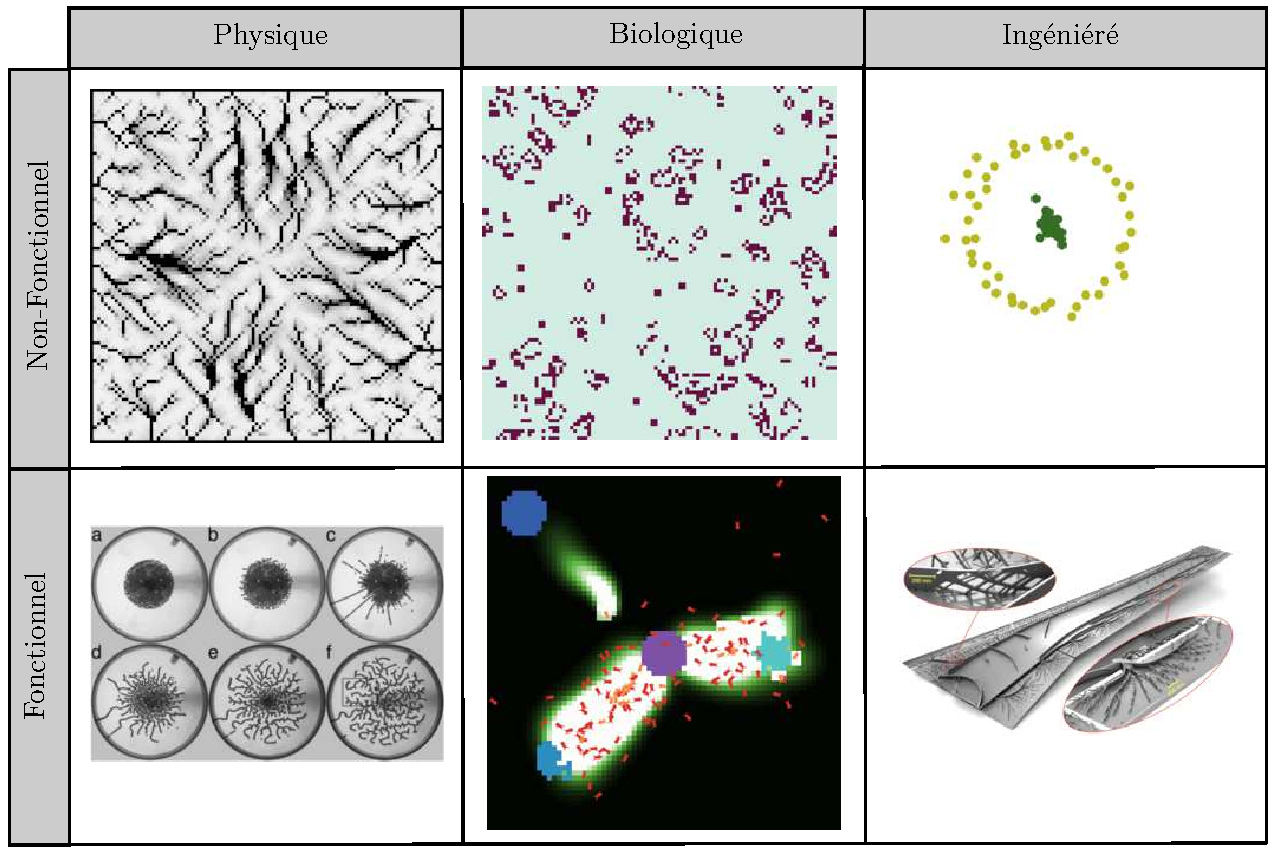
\includegraphics[width=\linewidth]{Figures/InterdiscMorphogenesis/intro_examples_fr.pdf}
		
		\medskip
		
		Nous donnons des illustrations dans trois disciplines typiques, et proposons une interprétation des caractères fonctionnels ou non (rendant les systèmes de la première ligne non-morphogénétiques en notre sens). Dans l'ordre de gauche à droite et de haut en bas : modèle d'érosion (bibliothèque NetLogo) ; jeu de la vie (voir~\ref{sec:epistemology}, bibliothèque NetLogo) ; \emph{Swarm chemistry} (particules abstraites ayant des règles de mouvement et d'interaction), implémenté à partir de \cite{sayama2007decentralized} ; arbotron (billes de métal sous l'influence d'un potentiel électrique) \cite{jun2005formation} ; modèle de fourmis (bibliothèque NetLogo) ; conception industrielle  \cite{Aage:2017aa}. Le jeu de la vie, s'il est utilisé comme ordinateur, peut avoir des aspects fonctionnels. De même l'arbotron ou le nuage de particules de la \emph{Swarm chemistry} peuvent être utilisés comme instruments. Tout est question de perspective dans laquelle le système est placé.
		
		\framecaption{\textbf{Examples of morphogenetic systems.}\label{frame:interdiscmorphogenesis:examples}}{\textbf{Exemples de systèmes morphogénétiques.} \label{frame:interdiscmorphogenesis:examples}}
	\end{mdframed}
\end{figure}
%%%%%%%%%%%%%%%%%%


\subsection{Discussion}{Discussion}

Avant de positionner l'utilité de la construction de ce concept par rapport à notre problématique générale, détaillons quelque développements potentiels propres à cet effort interdisciplinaire.


\subsubsection{Towards a more systematic construction}{Vers une construction systématique}

\bpar{
Our work relies for now on a broad but not \emph{systematic} review, in the sense of the methodology used for example in therapeutic evaluation, and where they play a role as important as primary studies, new knowledge being created through systematic comparison of results and meta-analysis. It would imply in our case an iterative approach :
}{
Ce travail repose pour l'instant sur une revue large mais non \emph{systématique}, au sens de la méthodologie utilisée en évaluation thérapeutique par exemple, et où elle joue un rôle aussi important que les études primaires, une nouvelle connaissance étant créée par la comparaison systématique des résultats et la meta-analyse. Cela impliquerait dans notre cas une approche itérative, en utilisant de manière couplée les différents outils et méthodes développés en~\ref{sec:quantepistemo}, selon le schéma suivant.
}

\bpar{
\begin{itemize}
\item Blind systematic review, without any a priori on the fields concerned and on the way to express the notion.
\item Extraction of main fields ; extraction of synonyms and close notions (such as we did here with autopoiesis and self-assembly for example ; if needed iteration of the first general review.
\item Systematic reviews specific to each field, as each one has its own bibliographical databases, specific ways of communication, etc.
\item Confrontation of each notion from one field to other fields.
\end{itemize}
}{
\begin{itemize}
\item Une revue systématique aveugle, sans aucun a priori des champs concernés ou des moyens d'exprimer la notion.
\item Extraction des champs principaux ; extraction des synonymes et notions proches (comme il a été fait ici avec l'autopoièse et la \emph{self-assembly} par exemple) ; si besoin itération de la première revue générale.
\item Revue systématique spécifique à chaque champ, puisque chaque a ses propres bases bibliographiques, moyens spécifiques de communiquer, etc.
\item Confrontation de chaque notion depuis un champ vers les autres.
\end{itemize}
}
 
L'objectif dans notre cas serait d'enrichir, comme nous l'avons déjà fait de manière préliminaire, mais systématiquement, le concept de morphogenèse urbaine.


\subsubsection{Quantitative Epistemology}{Epistemologie quantitative}

\bpar{
Our position may be also strengthen by quantitative approaches to literature analysis. With text-mining, keywords and concept extraction from abstracts (or even full texts) is possible, and would allow to confront our qualitative analysis to empirical data, by answering questions such as: is a concept indeed central, or what concept is used the same way in most disciplines. \cite{chavalarias2013phylomemetic} for example reconstructs scientific fields from the bottom-up through text-mining, and studies their lineage and dynamics in time. An other approach would be an iterative extraction of concept, by an algorithmic systematic review such as the one done in~\cite{raimbault2015models}.
}{
Notre position peut également être renforcée par des approches quantitatives à l'analyse de la littérature. Avec la fouille de texte, l'extraction de mots-clés et de concepts à partir des résumés (ou même des textes complets) est possible, et devrait permettre de confronter notre analyse qualitative à la réalité empirique, en répondant à des questions telles que : un concept est-il central, ou quel concept est utilisé de la même façon dans la plupart des disciplines. \cite{chavalarias2013phylomemetic} par exemple reconstruisent des champs scientifiques par le bas par une analyse textuelle, et étudie leur lignée et dynamique dans le temps.
}

% Une autre approche peut être la construction itérative des concepts, par une revue systématique algorithmique comme celle faite en chapitre~\ref{ch:modelinginteractions}.


\subsubsection{Transfer of Knowledge between fields}{Transfert de connaissances}


\bpar{
Concrete applications of our framework include potential transfer of knowledge between fields. As biological systems inspire system architecture in morphogenetic engineering, or as the use of gravity models inspired from physics have flourishing applications in geography, we think that trying to decline the general framework in specific disciplines may bring analogies or new models that would have been difficult to formulate otherwise.
}{
Les applications concrètes de ce cadre incluent un transfert potentiel de connaissances entre champs. Comme les systèmes biologiques inspirant l'architecture en \emph{morphogenetic engineering}, ou comme l'usage des modèles gravitaires inspirés par la physique a eu des applications riches en géographie, nous postulons que les tentatives de déclinaison du cadre dans des disciplines spécifiques peuvent favoriser des analogies ou d'autres modèles qui auraient été difficiles à formuler autrement.
}




\stars





